\documentclass[11pt]{article}
\usepackage[utf8]{inputenc} % use a civilized charset
\usepackage[T1]{fontenc}
\usepackage[letterpaper,left=3cm,right=3cm,top=3cm,bottom=3cm]{geometry}
\usepackage[english]{babel} % hon hon hon
\usepackage{hhline}% double underline
\usepackage{amsmath} % Math symbols
\usepackage{amsfonts}
\usepackage{amssymb}
\usepackage{graphicx}

\usepackage[bookmarksopen=true, hidelinks]{hyperref}
\usepackage{bookmark}
\usepackage[toc,page]{appendix}
\usepackage{url}
\usepackage{color}
\usepackage{shadow}
\usepackage{fancybox}
\usepackage[babel=true,autostyle=false, style=english]{csquotes}
\MakeOuterQuote{"} % automatically render quotes correctly

\usepackage{pxfonts}
\usepackage{parskip} % remove paragraph indent and add empty line between paragraphs

\newtheorem{thm}{Theorem}[section] 
\newtheorem{coro}{Corollary}[section]
\newtheorem{lem}{Lemma}[section]
\newtheorem{prop}{Proposition}[section]

\def\N{\mathbb{N}}
\def\R{\mathbb{R}}
\def\Q{\mathbb{Q}}
\def\Z{\mathbb{Z}}
\def\C{\mathbb{C}}

\author{I. Rhomboid\textsuperscript{1}}
\date{April NaN, 2025}

\title{Can one hear the shape of gender?}


%\bibliographystyle{plain} 
\pagestyle{plain}
\pagenumbering{gobble}

\begin{document}
\maketitle
{
\small
% Enter affiliation(s) here
\textsuperscript{1} Department of Mathematics, EAIOT\footnote{EleutherAI Discord \#off-topic}
}

\begin{abstract}
    Prior work showed that the modal human body has seven holes, irrespective of biological gender, which showed that gender is not a topological invariant. We conjecture that genders can be classified according to torsion and curvature, up to rigid motion, but that only spectral information is not enough. We check this conjecture empirically by training a machine learning model to classify meshes of male/female bodies based on topological and geometric features, and compute pairs of non-isogender isospectral bodies.
\end{abstract}

\section{Introduction}
The human body is known to display a wide range of shapes while having broadly the same general topology. This intuition was formalized in \cite{VsauceHoles} which first gave a rigorous proof that the modal human body is homeomorphic to a seven-holed torus. Their proof also showed that the number of holes in the human body does not depend on biological gender, meaning that gender is not a topological invariant.

In this work, we investigate whether biological gender can be characterized as a geometric invariant. We investigate this problem empirically using a dataset of meshes of human bodies generated from high quality scans \cite{Yang2014}. We generate several feature sets from these meshes based on topological, geometric and spectral information and train machine learning (ML) models to classify genders using these feature sets.

\section{Related work}

\subsection{Gender independence of topological genus}

\begin{figure}
    \centering
    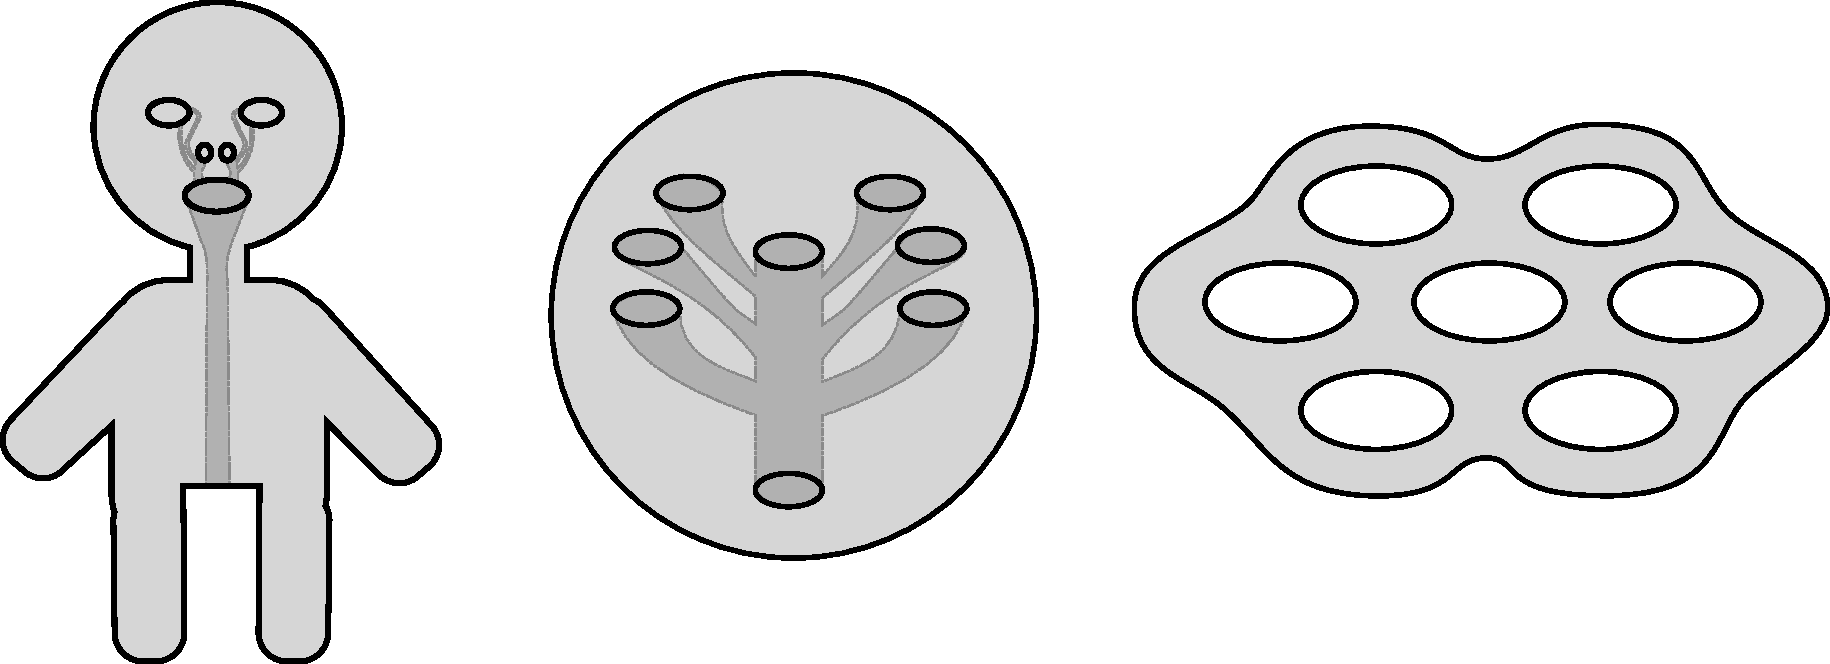
\includegraphics[width=.9\textwidth]{../plots/human-torus.pdf}
    \caption{Schematic illustration of a continuous transformation of a human body into a seven-holed torus.} \label{fig:torus}
\end{figure}

We restate here the proof that the modal human body is homeomorphic to a seven-holed torus. By hole, we mean a \textit{through-hole}, like the handle of a cup, through which a string could be passed. Cavities like the inside of a cup are \textit{blind holes}, which can be continuously filled up, and are therefore topologically irrelevant.

The most obvious hole in the human body is the digestive track, which connects the mouth to the rectum. The nostrils form two additional through-holes connected to the mouth cavity. In addition, the \textit{lacrimal canaliculi} (lacrimal ducts) connect the eyelids through the \textit{lacrimal puncta} to the nose. There is one duct per eyelid, adding four through-holes together, bringing the total to seven holes. Figure \ref{fig:torus} shows an illustration of the continuous deformation of a human body into a seven holed torus.

Other holes like the ears and urinary tract are in fact blind holes not connected to the holes listed in the previous paragraph. In addition, we ignore cavities located inside the human body, such as the brain cavity or the circulatory system. Importantly, the reproductive organs do not contribute any through-holes, which implies that biological gender is not a topological invariant.

It is important to note that seven is only the \textit{most common} number of through-holes in the human body. Any other holes resulting from injury, or cosmetic modifications (such as ear rings or piercings) will add to this count. In addition, people can be born with additional lacrimal puncta \cite{Saleh2021}. While it might be argued that holes made for cosmetic purposes could be used to determine one's gender, it would only do so imperfectly, as the practice of body piercing varies across cultures, and is not restricted to a single gender.

\section{Methods}

\subsection{Differential Geometric approaches to anatomy}

We model the surface of the human body as a \textit{Riemannian manifold} $\mathcal{M}$. Riemannian surfaces can be completely described (up to isometry) by their Gaussian curvature $K$, which is a scalar quantity defined for each point $p \in \mathcal{M}$ as $K = \kappa_1 \kappa_2$, where $\kappa_i$ denote the \textit{principal curvatures} at point $p$. Positive curvature indicates that $\mathcal{M}$ looks like the surface of a sphere around $p$, while negative curvature indicates that it looks like a saddle surface. If $K=0$, $\mathcal{M}$ is said to be \textit{flat} at $p$, meaning that around $p$ it looks like a sheet of paper that could be flattened out.

We claim that Gaussian curvature can be used to identify biological gender, as secondary sexual characteristics in humans include different distributions of fat and muscle tissue, notably around the hips and breasts for females, and shoulders, larynx and belly for males. These are not the only factors in the variation of body shapes, but we argue they are among the most important ones.

\subsection{Dataset}

In the absence of a complete mathematical description of the human body that would allow for a formal proof of our claim, we instead adopt a data-driven approach. We use the dataset of \cite{Yang2014}, which consists of 3048 polygonal meshes obtained from scans of human subjects. Each mesh in the dataset is fit to the same topology with 12500 vertices and 25000 faces. The dataset is split equally between female and male subjects. We process this dataset by smoothing each mesh to eliminate any artifacts which may erroneously change the curvature at specific points.

\subsection{Topological Features}

\begin{figure}
    \centering
    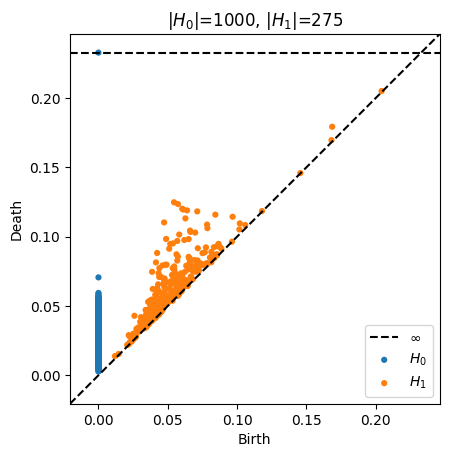
\includegraphics[width=0.3\textwidth]{../plots/persistence-diagram.png}
    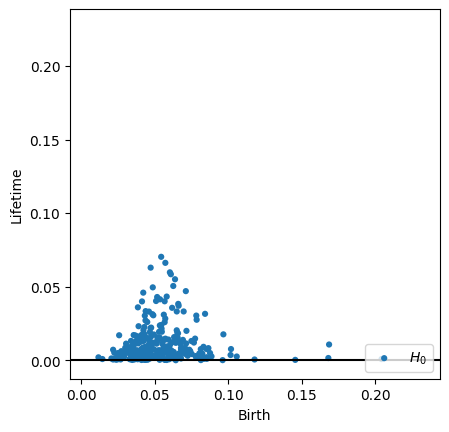
\includegraphics[width=0.3\textwidth]{../plots/birth-lifetime.png}
    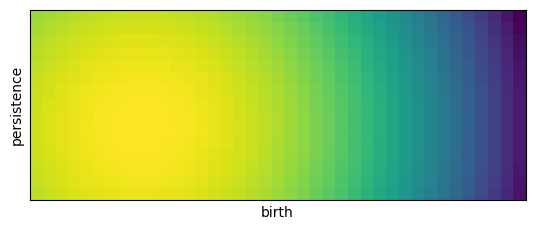
\includegraphics[width=0.3\textwidth]{../plots/persistence-image.png}
    \caption{Typical topological features obtained from persistent homology on a mesh from the dataset.}
    \label{fig:tda}
\end{figure}

We use the Scikit-TDA package \cite{scikittda2019} to compute topological features from the vertex point cloud of each mesh. Specifically, we use Persistent Homology to record the emergence of one dimensional cycles over the Vietoris-Rips filtration of the mesh. Due to the large number of vertices and the high computational cost of persistent homology, we only use a small subset of 1000 vertices chosen randomly.

From the persistence homology process, we obtain a collection of birth and death times for each cycle that emerged during the filtration. Most such cycles are spurious and die shortly after their birth. Cycles that persist for a longer duration are typically indicative of actual topological features of the point cloud.

To turn the output of persistent homology into convenient features for statistical analysis, we take  figure \ref{fig:tda}) and take a two-dimensional histogram of the resulting point cloud over a coarse grid (third panel of figure \ref{fig:tda}). This yields $465$ scalar values for each mesh, which we use as features for our analysis.

\subsection{Geometric Features}

Given a triangular mesh approximating a Riemannian manifold, we can estimate the Gaussian curvature at a vertex $v$ by computing the \textit{angle defect} at $v$, defined as $\pi - \sum_i \theta_i$, where the numbers $\theta_i$ are the angles at $v$ for each triangle containing $v$. The interpretation of angle defect is the same as the gaussian curvature $K$. We compute the angle defect at each vertex to obtain our first (\textit{intrinsic}) geometric feature set.

In addition to curvature via the angle defect, we also use the euclidean coordinates of each vertex, concatenated into a single vector to form our second (\textit{extrinsic}) geometric feature set. In both cases, our geometric feature sets have many more variables than observations, which may pose a problem for statistical methods.

\subsection{Spectral Features}

A famous problem in differential geometry, posed by Kac in 1966 \cite{Kac1966}, asks whether the spectrum of the Laplace-Beltrami operator\footnote{The Laplace-Beltrami operator, also known as the diffusion operator, has a central role in harmonic analysis via the Laplace and Poisson equations.} of a manifold can be used to identify it. Physically, this can be interpreted as whether the shape of a drum can be identified by listening to the frequencies it emits as it vibrates upon being hit.

This question was answered in the negative by the discovery of non-isomorphic manifolds with the same Laplacian spectrum \cite{Buser1994}. Inspired by this classical result, we ask whether the spectrum of the Laplace-Beltrami operator can be used to differentiate between genders, or in more poetic words, "\textit{Can one hear the shape of gender?}". Physically, one should imagine taking a semi-rigid shell of a human body and trying to identify its gender by listening to the sounds it makes as it vibrates.

We compute the eigenvalues of the discrete approximation of the Laplace-Beltrami operator on the meshes in our dataset. Since computing the full spectrum of large (sparse) matrices is computationally expensive, we only compute the 20 largest eigenvalues in magnitude. This choice is suboptimal, however, as the largest eigenvalues correspond to the higher frequency harmonic functions on the manifold, which may be less informative than the lower frequencies.

\section{Results}

\begin{table}
    \centering
    \begin{tabular}{c|c|c}
        & \textbf{Train accuracy} & \textbf{Test accuracy}\\ \hline
    Topological features & 0.5 & 0.5 \\
    Angular Defect & 1.0 & 1.0 \\
    Vertex Coordinates & 0.5 & 0.5 \\
    Spectral Features & 0.5 & 0.5\\
    \end{tabular}
    \caption{Train and test accuracies across feature sets} \label{tab:results}
\end{table}

We use each of the feature sets described in the previous section as features for performing logistic regression to predict the gender of each mesh\footnote{The code to reproduce our analyses can be found at \url{https://github.com/irregular-rhomboid/gender-geometry}}. The results are summarized in table \ref{tab:results} We find that only the angular defect allows perfect classification, while all other feature sets perform as well as random chance. We interpret this as evidence to our claim that gender can be characterized using Gaussian curvature.

To further investigate this result, we perform principal component analysis on our angle defect dataset. As seen in figure \ref{fig:pca}, we find that nearly all of the variance across the dataset is explained by the first two components, and that both biological genders are clustered in the second component and perfectly linearly separated, which explains the excellent classification performance of the model trained on angular defect.

Regarding our other conjectures, we observe that the numerical ranks of feature matrices of both the topological and spectral datasets are equal to one. This indicates that the rows of these datasets are all essentially the same, which serves as evidence towards our claims that neither topological nor spectral information is enough to characterize gender.

\begin{figure}
    \centering
    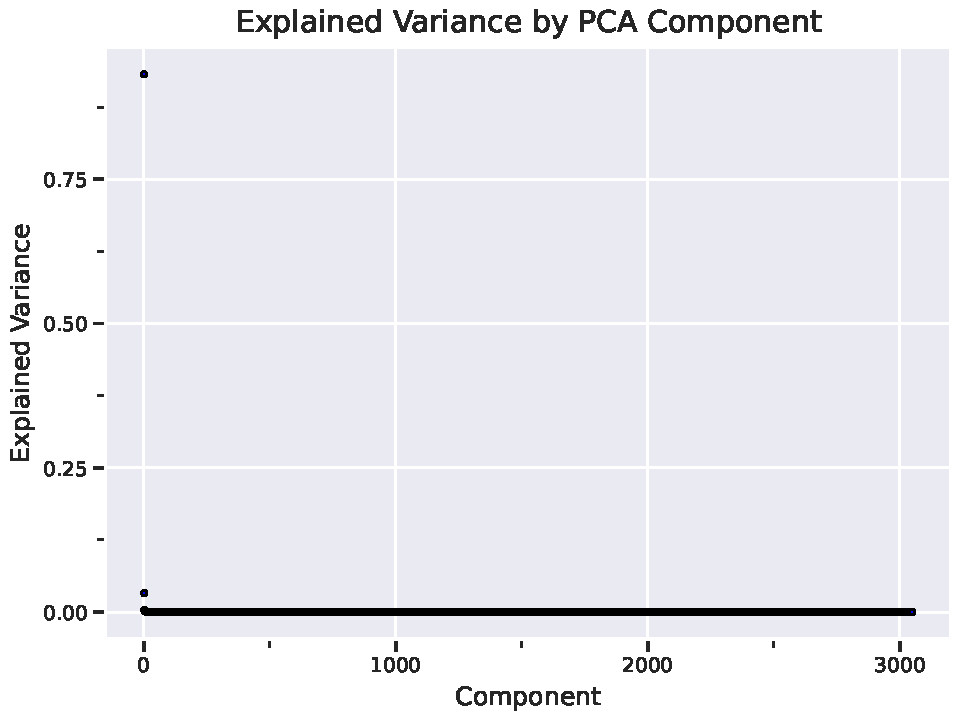
\includegraphics[width=.45\textwidth]{../plots/pca_variance.pdf}
    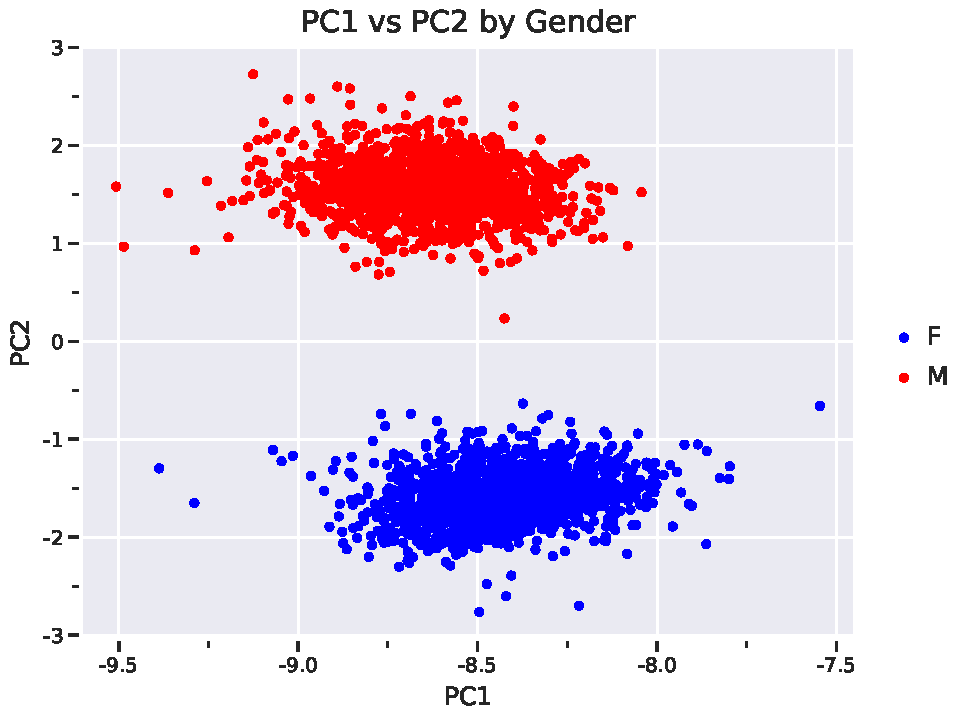
\includegraphics[width=.45\textwidth]{../plots/pca_components.pdf}
    \caption{Principal Component Analysis of the Angle Defect feature set}
    \label{fig:pca}
\end{figure}

\section{Discussion}

In this work, we have uncovered empirical evidence that biological gender can be characterized using the Gooseian curvature of the outer surface of the human body. While this is encouraging and may serve as a stepping stone to a formal mathematical proof, it is important that we state the limitations of our results.

First, our discussion thus far has only been about \textit{biological gender}, which as our results show, is only skin deep, and besides is only a narrow subcategory of gander as a whole. To our knowledge, a proper mathematical description of the broader question of gender remains to be seen, and we do not believe that the tools used here are enough for this task, which may necessitate more advanced tools from non-commutative geometry and category theory to account for its highly nontrivial complexity. We leave such worthy task to more capable hands.

Second, our statistical analysis of the available data was restricted to logistic regression due to limited computational resources and time constraints. More recent models such as K-Nearest-Neighbors \cite{Knns} or Support Vector Machines \cite{SVMs} may be used by further work to improve the accuracy on the other feature sets.

\bibliographystyle{unsrt} 
\bibliography{sources}

\end{document}